\documentclass[a4paper]{article}
\setlength{\parskip}{\baselineskip}

% First load extension packages
\usepackage[a4paper,margin=25mm]{geometry}    % page layout
\usepackage{setspace} \onehalfspacing         % line spacing
\usepackage{amsfonts,amssymb,amsmath}         % useful math extensions
\usepackage{graphicx}                         % graphics import
\graphicspath{{../figs/}}
\pdfpageattr{/Group << /S /Transparency /I true /CS /DeviceRGB>>}
\usepackage[colorlinks=true, allcolors=black]{hyperref}
\usepackage{hhline}
\usepackage{subcaption}
% Change paragraph indentation
\setlength{\parskip}{10pt}
\setlength{\parindent}{0pt}
\usepackage[toc]{multitoc}
%\renewcommand*{\multicolumntoc}{2}
\setlength{\columnsep}{36pt}
% User-defined commands
\newcommand\numberthis{\addtocounter{equation}{1}\tag{\theequation}}
% topmatter
\title{\vspace{-50pt}\huge\bfseries Developing a Coarse-Grained Model
to Investigate Long-Term Climate Behaviour}

\author{Liam Wheen \\ Supervised by Dr O.\ Benjamin}

\date{\today}
\pagenumbering{gobble}
% main body
\begin{document}
\begin{titlepage}
\maketitle
\hrule
\vspace{-10pt}
\begin{abstract}
\noindent
This is the abstract.
\end{abstract}
\hrule
\end{titlepage}
%\vspace{20pt}
\newpage
\pagenumbering{gobble}
%\begin{spacing}{0.6}
\tableofcontents
%\end{spacing}
\newpage
\pagenumbering{arabic}
\section{Introduction}
\section{Budyko Model}
The Budyko model is an energy balance model (EBM) that explores the positive
feedback effect of polar ice cap albedo. The increased reflectivity of polar
ice caps reduces the net energy that Earth can absorb from the sun across these
regions. If a sufficient amount of Earth's surface is covered in ice, 
global temperatures drop, and the polar ice caps advance towards the equator.
Conversely, if the ice caps only exist at very high latitudes, then the reduced
reflectivity will allow Earth to absorb more heat, and temperatures to rise,
leading the ice-line to recede further.

A number of assumptions are made in order for this EBM to work. Temperature
is modelled as varying only across latitude, reducing the domain of the
system from a spherical surface, to a 1-dimensional temperature profile. In
order to simplify integrals that span the latitudes, the
domain is described using $y = \sin(\varphi)$, where $\varphi$ is latitude.
To simplify the system further, the Earth is treated as an entirely water-based
planet. This allows for the differences in ground reflectivity to be ignored,
focusing only on the albedo of water and ice. The Earth is also modelled as
symmetric across the equator, allowing for only one half of the domain to be
considered, i.e. $y \in [0,1]$.

The dynamical equation for temperature consists of three components. They
describe the flow of energy into, out of, and around Earth.
The first of these is incoming solar radiation, expressed by the term
$Q_\varepsilon s(y) (1-\alpha_\eta(y))$. This consists of the average yearly insolation reaching
Earth, $Q_\varepsilon$, which varies according to the eccentricity of Earth's
orbit, $\varepsilon$, such that $Q_\varepsilon = Q_0/\sqrt{(1-\varepsilon^2)}$ where $Q_0$ is
a constant found using empirical data. This insolation is then distributed
according to latitude, using the function
\[
  s(y) = 1+ \frac{1}{2}c_\beta(3y^2-1),
\]
where $c_\beta = \frac{5}{16}(3\sin^2\beta - 2)$ and $\beta$ is obliquity.
This is finally multiplied by $(1-\alpha_\eta(y))$, which describes the degree
to which heat is absorbed at a given latitude. This depends on the albedo of
the surface, which in this case is either water or ice. The albedo over the
domain is therefore given as
\[
  \alpha_\eta(y) = \begin{cases} \alpha_1, & y<\eta\\
                                 \alpha_2, & y>\eta\\
                                 \frac{1}{2}(\alpha_1+\alpha_2), & y=\eta
                   \end{cases},
\]
where $\eta$ is the location of the ice lice and $\alpha_1$ and $\alpha_2$ are
also determined through empirical data. This results in less heat being
absorbed over the range where ice is present due to the increased reflectivity.

The next component of the equation is the outgoing infra-red radiation.
This is approximated to linearly depend on the temperature of Earth to give
\[
  A+BT(y,t).
\]
Although the energy flow occurring within Earth's atmosphere is far more
complex, satellite data was used to establish the net flow of heat from Earth
to the first order \cite{linear_reradiation}.

The final component describes the transport of energy around Earth, from
the hot equator to the relatively cooler poles. The heat transport at a given
latitude is determined by the difference in temperature at this latitude and
the global average temperature, written as
\[
  C(\bar{T}-T(y,t)),
\]
where
\[
  \bar{T} = \int_0^1 T(y,t) \,\mathrm{d}t.
\]
By calculating the equilibrium solution for the temperature, $C$ can be chosen
such that the equilibrium matches current climatic conditions. Tung's work on
this yielded the relation $C=1.6B$ \cite{tung2007topics}.
Combining these components of heat flow gives the dynamical equation for temperature to be
\[
  R\frac{\partial T(y,t)}{\partial t} = \underbrace{Qs(y) (1-\alpha_\eta(y))}_{\text{Insolation}}
  - \underbrace{(A+BT(y,t))}_{\text{Reradiation}}
  + \underbrace{C(\bar{T}-T(y,t))}_{\text{Transport}},
\]
where $R$ represents the heat capacity of Earth's surface.

A dynamic ice line was later introduced to the model by Widiasih
\cite{widiasih2013}, such that
\[
  S\frac{\mathrm{d}\eta(t)}{\mathrm{d}t} = T_\eta(\eta,t) - T_{\mathrm{ice}}
\]
where $T_{\mathrm{ice}}$ is an estimate for the critical temperature at which
an ice sheet can form. Budyko
[Here discuss the introduction of the dynamic iceline from widiasih, the
  dynamics of the model, the equilibrium points, the stability, how this
  doesn't get effected by the milankovitch params much at all, the lack of any
  oscillation (which I believe would be impossible anyway given the equations
  formulation), the slow and fast dynamics of the temp and iceline
respectively (as shown in the figure).]
[Also introduce Milankovitch properly and how each orbital parameter is defined
(especially precession). Maybe move Table of orbital params up to milankovitch
section]
  
\begin{figure}
\centering
\begin{subfigure}{.4\textwidth}
  \centering
  \includegraphics[width=\linewidth]{demo_budyko_0.pdf}
  \caption{0 Years}
\end{subfigure}%
\begin{subfigure}{.4\textwidth}
  \centering
  \includegraphics[width=\linewidth]{demo_budyko_1.pdf}
  \caption{10 Years}
\end{subfigure}
\begin{subfigure}{.4\textwidth}
  \centering
  \includegraphics[width=\linewidth]{demo_budyko_2.pdf}
  \caption{3000 Years}
\end{subfigure}%
\begin{subfigure}{.4\textwidth}
  \centering
  \includegraphics[width=\linewidth]{demo_budyko_3.pdf}
  \caption{10\,000 Years}
\end{subfigure}
\caption{Snapshots of a Budyko simulation starting with 0$^\circ$C at all
latitudes and the ice line at $y=0.5$. The orbital parameters used are shown in
Table \ref{tab:orbital_params}. We first see the temperature profile
equilibrate within 10 years. The ice line then recedes 
towards the stable equilibrium point at $y=0.9544$, getting within 3\% of this
value after 10\,000 years.}
\label{fig:budyko_demo}
\end{figure}


\section{Insolation}
To implement an asymmetrical version of the Budyko model, the difference
between the northern and southern hemispheres must first be established. We
will therefore be looking at the variation of insolation over different
latitudes. Insolation is solar irradiance integrated over time, however we are
usually interested in the average insolation over a given time period, hence
the units for both irradiance and average insolation are Wm$^{-2}$. We will
first look at average daily insolation to see how this varies throughout a
year, then a yearly average will be used to investigate long-term changes to
insolation across different latitudes. All simulations that depend on the Milankovitch cycles take this
data from Laskar \cite{laskar2004}.

To model the average insolation over a chosen period, we first express
the irradiance arriving at a given point on Earth, in terms of the orbital
parameters, latitude, and longitude. We will use two frames of reference to
derive this expression. The ``ecliptic frame''
places Earth's orbit in the $x$-$y$ plane with the $x$-axis directed along the
orbit's semi-major axis towards the aphelion (the farthest point from the sun
on Earth's orbit). Using a sun centred coordinate system, we can represent
Earth's position using polar coordinates $\theta$ and $r$. The ``Earth-fixed
frame'' changes with Earth, according to obliquity and precession. With an
Earth centred coordinate system in this frame, we can utilise spherical
coordinates to describe a point on Earth with the unit vector
\[
  \mathbf{u} = \begin{bmatrix}\cos\varphi\cos\gamma\\\cos\varphi\sin\gamma\\\sin\varphi\end{bmatrix}
\]
which points towards latitude $\varphi$ and longitude $\gamma$ on Earth, hence
$(\varphi,\gamma)$ = $(0,0)$ lies along the positive $x$-axis, whilst the north
pole aligns with the positive $z$-axis.

We now introduce two matrices to describe the rotation of these Earth centred axes,
from the ecliptic frame to the Earth fixed frame. These are
\[
  U_{\beta} = \begin{bmatrix}\cos{\beta} & 0 & \sin{\beta}\\0 & 1 & 0\\-
  \sin{\beta} & 0 & \cos{\beta}\end{bmatrix},\quad\quad
  U_{\rho} = \begin{bmatrix}\cos{\rho} & - \sin{\rho} & 0\\\sin{\rho} &
  \cos{\rho} & 0\\0 & 0 & 1\end{bmatrix}
\]
for obliquity and precession respectively. $U_{\beta}$ acts first,
rotating around the ecliptic $y$-axis, followed by $U_{\rho}$, acting
around the ecliptic $z$-axis.

We now require an expression for irradiance at a given point ($\varphi,\gamma$) given
$\theta, r, \beta,$ and $\rho$. For this we will use an Earth centred
coordinate system in the Earth fixed frame.

Firstly, we express the irradiance at Earth's atmosphere as the total solar
output $K$ distributed over the surface area of an imagined sphere with a radius
equal to Earth's distance from the sun. This gives
\[
  \frac{K}{4\pi r^2}\,\,\mathrm{Wm^{-2}}.
\]

The irradiance at ($\varphi,\gamma$) is proportional to the cosine of
the angle between $\mathbf{u}$ and the vector that
points from Earth to the sun, $\mathbf{n}$. This vector uses $\theta$, Earth's angle
around the sun in ecliptic polar coordinates, expressed in this frame as
\[
  \mathbf{n} = \left(U_{\rho}U_{\beta}\right)^{-1}\begin{bmatrix}-\cos\theta\\-\sin\theta\\0\end{bmatrix} = 
  \begin{bmatrix}-\cos{\beta} \cos(\rho - \theta)\\
  \sin(\rho - \theta)\\-\sin{\beta} \cos(\rho -\theta)\end{bmatrix}.
\]
Multiplying the scalar product of these two unit vectors by the irradiance at
the atmosphere gives
\[
  \begin{split}
    I(r,\theta,\beta,\rho,\varphi,\gamma) &= \frac{K}{4\pi
    r^2}\,\mathbf{u}^\top\mathbf{n}\\
  &=\frac{K}{4\pi r^2}
  \begin{bmatrix}\cos\varphi\cos\gamma\\\cos\varphi\sin\gamma\\\sin\varphi\end{bmatrix}^\top
  \begin{bmatrix}-\cos{\beta} \cos(\rho - \theta)\\
  \sin(\rho - \theta)\\-\sin{\beta} \cos(\rho -\theta)\end{bmatrix}\\
  &= \frac{K}{4\pi r^2}[(\sin{\gamma}\sin{(\rho - \theta)}-\cos{\beta} \cos{\gamma}
    \cos{(\rho-\theta)})\cos{\varphi}
  -\sin{\beta}\sin{\varphi} \cos{(\rho -\theta)}].
\end{split}
\]

Note this expression is only valid for positive values, since the irradiance value
for the dark side of Earth will be negative, when it should be 0. To
calculate the average daily insolation, we can treat the orbital parameters as
constant and integrate with respect to longitude $\gamma$ over the range
$[0,2\pi]$. However, since this
expression is only valid for positive values,
we must either augment our expression for irradiance, $I$, to be the piecewise function Max$(0,I)$, or define the limits such
that we only integrate over the range of longitudes that receive sunlight.
Through simulation, the former approach was found to be far more
computationally costly as the piecewise needed evaluating at every step of the
integration, whereas the piecewise limits only need to be calculated once. 

To find these limits in terms of the orbital parameters, we consider a plane
passing through the origin, separating the light and dark hemispheres of Earth,
rotating so that its normal vector always points towards the sun. The plane can
therefore be expressed as
\[
  ax+by+cz=0,
\]
where $a$, $b$, and $c$ are the components of $\mathbf{n}$.

Next consider a circle of constant latitude $\varphi$, lying parallel to the
$x$-$y$ plane such that
\[
  x^2+y^2 = \cos^2\varphi.
\]
Note this is using a unit sphere for convenience since longitude is
invariant with size.
The intersections of this circle with the plane separating day and night
indicate the limits over which integration should be performed for the given
latitude and orbital parameters. An example of this can be seen in Figure
\ref{fig:circ_plane_intercept}.
\begin{figure}
  \centering
  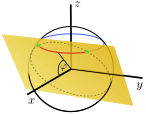
\includegraphics[width=0.6\linewidth]{circ_plane_intercept.pdf}
  \caption{Diagram showing the day-night plane (yellow) that passes through the
    origin at Earth's centre and rotates to face the sun, and the circle of
    constant latitude $\varphi$. The points where the circle intersects the plane
    (green) indicate the range of longitudes for which sunlight will reach Earth
  at latitude $\varphi$ (red) whilst longitudes on the opposite side of the
plane (blue) are in darkness so receive no insolation.}
  \label{fig:circ_plane_intercept}
\end{figure}

Using the final condition that 
\[
  z = \sin\varphi,
\]
we find the two intersection points to be
\[
  \boldsymbol{\mu}_{0,1}=\frac{1}{a^2 + b^2}\begin{bmatrix}- a c \sin{\varphi}\mp b
    \sqrt{\left(a^2+b^2\right) \cos^2{\varphi}- c^2 \sin^2{\varphi}}\\
  - b c \sin{\varphi}\pm a \sqrt{\left(a^2+b^2\right) \cos^2{\varphi}
  - c^2 \sin^2{\varphi}}\\
(a^2 + b^2)\sin{\varphi}\end{bmatrix}.\numberthis
\label{eq:integration_limits}
\]

Looking at (\ref{eq:integration_limits}), we see there are two real
solutions when the discriminant, 
\[
  \left(a^2+b^2\right) \cos^2{\varphi} - c^2 \sin^2{\varphi} = \Delta,
\]
is positive.

If $\Delta \le 0$, then there is either no intersection between the circle
and the plane, or only one. Hence the entire circle of latitude $\varphi$ will lie
on the dark, or light, side of the plane.

To determine which side it is, we return to the scalar product
$\mathbf{u}^\top\mathbf{n}$ where $\mathbf{u}$ will point to some part of the
circle and $\mathbf{n}$ points from Earth to the sun. If no intersection has
occurred, and $\mathbf{u}^\top\mathbf{n}$ is positive, then this point, and the
entirety of the circle lies within sunlight, whilst a negative product 
corresponds to darkness. To simplify this calculation, we use choose
$(\varphi,0)$ for the point on the circle, giving
\[
  \mathbf{u}^\top\mathbf{n}\,\bigr|_{\gamma=0} = -\cos\left(\beta - \varphi
  \right) \cos\left(\rho - \theta \right).
\]

In the rare case that this is exactly equal to 0, a different point on the
circle would be chosen.

The intersection points, $\boldsymbol{\mu}_0$ and $\boldsymbol{\mu}_1$, are
currently expressed in Cartesian coordinates. For the corresponding longitudes
we use the definition $\gamma = \arctan\left(\frac{y}{x}\right)$. We can now
express the longitudinal limits in piecewise form as
\[\gamma_0 = \begin{cases}
    \arctan\left(\frac{\mu_{0y}}{\mu_{0x}}\right), & \Delta>0\\
    0, & \Delta\le 0
  \end{cases},
  \quad\quad\quad
  \gamma_1 = \begin{cases}
    \arctan\left(\frac{\mu_{1y}}{\mu_{1x}}\right), & \Delta>0\\
    2\pi, &\Delta\le 0 \land\mathbf{u}^\top\mathbf{n}\,\bigr|_{\gamma=0}> 0\\
    0, &\Delta\le 0 \land\mathbf{u}^\top\mathbf{n}\,\bigr|_{\gamma=0}< 0
  \end{cases},
\]
where the limits become either $[0,2\pi]$ or $[0,0]$ if the given latitude lies
entirely in day or night respectively.

The calculation for daily average insolation is therefore
\[\begin{aligned}
  Q_{\mathrm{day}} &= \frac{1}{2\pi} \frac{K}{4\pi
  r^2}\int_{\gamma_0}^{\gamma_1} (\sin{\gamma}\sin{(\rho - \theta)}-\cos{\beta} \cos{\gamma}
    \cos{(\rho-\theta)})\cos{\varphi} -\sin{\beta}\sin{\varphi} \cos{(\rho
    -\theta)}\,\mathrm{d}\gamma\\ 
  &=\frac{K}{8\pi^2r^2}[(\gamma_{0} - \gamma_{1}) \sin{\beta}
  \sin{\varphi} \cos{\left(\rho - \theta \right)} +
  (\sin{\gamma_{0}} \cos{\beta}
  \cos{\left(\rho - \theta \right)} - \sin{\gamma_{1}} \cos{\beta} \cos{\left(\rho - \theta \right)}\\
&\quad\quad\quad\quad\quad\quad + \sin{\left(\rho - \theta \right)} 
\cos{\gamma_{0}} - \sin{\left(\rho - \theta
\right)} \cos{\gamma_{1}} ) \cos{\varphi}].
\end{aligned}
\]
With this expression, we can see how average daily insolation changes
across the globe during a year. Figure \ref{fig:daily_ave_insol_all_lats} shows
how insolation varies over a year across latitudes with current orbital parameters
as well as how it is expected to look 1.0167$\times10^6$ years in the future,
when eccentricity is more extreme at 0.0582. This point in the future was chosen because the
obliquity and precession are both within 2\% of
present values, allowing us to isolate the impact of eccentricity on the
distribution of insolation.
\begin{table}[h]
  \centering
  \caption{Earth's orbital parameters in the year 2000.}
\label{tab:orbital_params}
\begin{tabular}{lllll}
  \multicolumn{1}{l|}{Eccentricity ($\varepsilon$)} & 0.0167 &  &  &  \\ \cline{1-2}
  \multicolumn{1}{l|}{Obliquity ($\beta$)}    & 0.4091 radians &  &  &  \\ \cline{1-2}
  \multicolumn{1}{l|}{Precession ($\rho$)}   & 2.9161 radians &  &  &  \\
\end{tabular}
\end{table}

When eccentricity is at its greatest, we can more clearly see the
asymmetry between the hemispheres during their summer solstices. These
occur at 170 and 352 days after aphelion for the southern and northern
hemispheres respectively. The southern hemisphere is shown to experience hotter
summers than the northern hemisphere. This is due to Earth's elliptical orbit
bringing it closer to the sun during the southern summer solstice, with the
perihelion occurring just 12 days later. The reduced distance from the sun
exposes Earth to greater irradiance, which is proportional to $1/r^2$.
Hence we can relate eccentricity to the inequality of the hemisphere's
peak insolation values. However, we will see that eccentricity also
effects the duration for which this insolation is experienced, cancelling out
the effect over a year period.
\begin{figure}
  \centering
  \includegraphics[width=\linewidth]{both_daily_ave_insolation_all_lats.pdf}
  \caption{Contours showing the daily average insolation arriving at
    the atmosphere for different latitudes over a year period. The left plot is
  based on current orbital parameters, as shown in Table
\ref{tab:orbital_params}, the right plot is how the insolation will be
distributed 1.0167$\times10^6$ years from now. At this time, eccentricity is close to its maximum value at 0.0582,
whilst precession and obliquity are similar to current values.}
  \label{fig:daily_ave_insol_all_lats}
\end{figure}

In order to investigate average yearly insolation over a long period we must
return to the expression for irradiance at a given point,
\[\begin{aligned}
  I &= \frac{K}{4\pi r^2}\mathbf{u}^\top\mathbf{n}\\
    &= \frac{K}{4\pi
    r^2}\begin{bmatrix}\cos\varphi\cos\gamma\\\cos\varphi\sin\gamma\\\sin\varphi\end{bmatrix}^\top
    U_{\beta}^{-1}U_{\rho}^{-1}\begin{bmatrix}-\cos\theta\\-\sin\theta\\0\end{bmatrix},
  \end{aligned}
\]
which is only valid for positive values of $I$.

It will be useful to define 
\[
  \begin{bmatrix}\cos\varphi\cos\gamma\\\cos\varphi\sin\gamma\\\sin\varphi\end{bmatrix}^\top
  U_{\beta}^{-1} = \begin{bmatrix}\sin{\beta} \sin{\varphi } + \cos{\beta}
  \cos{\gamma} \cos{\varphi}\\\sin{\gamma} \cos{\varphi }\\\cos{\beta }\sin{\varphi} - \sin{\beta} \cos{\gamma}
\cos{\varphi} \end{bmatrix}^\top =
  \begin{bmatrix}\cos\hat{\varphi}\cos\hat{\gamma}\\\cos\hat{\varphi}\sin\hat{\gamma}\\\sin\hat{\varphi}\end{bmatrix}^\top,\numberthis
  \label{eq:u_hat_definition}
\]
where $\hat{\varphi}$ and $\hat{\gamma}$ can be visualised as the latitude and
longitude measured not from the north pole, but from the $z$-axis in the
ecliptic frame. The irradiance at a given point can therefore be written as
\[
  I = \frac{K}{4\pi r^2}\begin{bmatrix}\cos\hat{\varphi}\cos\hat{\gamma}\\\cos\hat{\varphi}\sin\hat{\gamma}\\\sin\hat{\varphi}\end{bmatrix}^\top 
  \begin{bmatrix} -\cos{\left(\rho - \theta \right)}\\\sin{\left(\rho - \theta
  \right)}\\0\end{bmatrix} = -\frac{K}{4\pi r^2} \cos\hat{\varphi}\cos{\left(\hat{\gamma} + \rho - \theta \right)}
\]
Treating the orbital parameters as fixed, the average insolation over a year
period, $P$, for a given point is
\[
  Q = \frac{1}{P}\int_0^P\frac{-K}{4\pi r^2}
  \cos\hat{\varphi}\cos{\left(\hat{\gamma} + \rho - \theta
  \right)}\,\mathrm{d}t,\numberthis
  \label{eq:yearly_insol_integral_dt}
\]
however, since $r$ and $\theta$ have a non-linear dependence on time, we shall
use $\theta$ as the variable of integration. Kepler's second law of planetary
motion states
\[
  \frac{\mathrm{d}t}{\mathrm{d}\theta} = \frac{Pr^2}{2\pi ab},
\]
where $a$ and $b$ are the semi-major and semi-minor axes of Earth's orbit
respectively.

Substituting $\theta$ for $t$ in (\ref{eq:yearly_insol_integral_dt}) now
gives
\begin{align}
    Q &=\frac{1}{P}\int_0^{2\pi}\frac{-K}{4\pi r^2}
    \cos\hat{\varphi}\cos{\left(\hat{\gamma} + \rho - \theta \right)}
    \frac{Pr^2}{2\pi a b}\,\mathrm{d}\theta\nonumber\\ 
    &=\frac{K\cos\hat{\varphi}}{8\pi^2
    a b}\int_0^{2\pi}-\cos{\left(\hat{\gamma} + \rho - \theta \right)}
    \,\mathrm{d}\theta.\label{eq:yearly_insol}
\end{align}
Since the expression for $I$ is only valid for positive values, the integral in
(\ref{eq:yearly_insol}) is equivalent to the positive area under $\cos\theta$ 
from 0 to 2$\pi$, which gives 2. The average yearly insolation is therefore
\[
  Q = \frac{K\cos\hat{\varphi}}{4\pi^2 a b}.
\]
Note that this quantity no longer depends on precession, which will be
explained shortly.

In order to attain an expression for average yearly insolation for just a given
latitude, we must also average over all longitudes. It will be of more use to
express this in the Earth-fixed frame, using the conventional latitude values.
For this we refer to (\ref{eq:u_hat_definition}), which defines
\[
  \sin{\hat{\varphi}} = \cos{\beta}\sin{\varphi} -
  \sin{\beta}\cos{\gamma}\cos{\varphi},
\]
hence
\[
  Q = \frac{K\sqrt{1 -\left( \cos{\beta}\sin{\varphi} -
  \sin{\beta}\cos{\gamma}\cos{\varphi}\right)^2}}{4\pi^2 a b}.
\]

We now average this over longitude to get
\[
  \frac{K}{4\pi^2 a b}\frac{1}{2\pi} \int_0^{2\pi}\sqrt{1 -\left( \cos{\beta}\sin{\varphi} -
  \sin{\beta}\cos{\gamma}\cos{\varphi}\right)^2}\,\mathrm{d}\gamma.
\]

In order to express this purely as a function of orbital parameters and
latitude, we use the relation $b = a\sqrt{1-\varepsilon^2}$, where
$\varepsilon$ is orbital eccentricity. Further, we know that Earth's semi-major
axis, $a$, remains essentially constant regardless of orbital parameters
\cite{laskar2004}. This gives the average yearly insolation for a given
latitude to be
\[
  Q_{\mathrm{year}}(\beta,\varepsilon,\varphi) = \frac{K}{8\pi^3 a^2 \sqrt{1-\varepsilon^2}}\int_0^{2\pi}\sqrt{1 -\left( \cos{\beta}\sin{\varphi} -
  \sin{\beta}\cos{\gamma}\cos{\varphi}\right)^2}\,\mathrm{d}\gamma.
\]

Importantly, this expression is even in $\varphi$, meaning that yearly
insolation is symmetric across the equator. This can be seen
in Figure \ref{fig:yearly_ave_insol_present} which uses current orbital
parameters shown given in Table \ref{tab:orbital_params}.
\begin{figure}
  \centering
  \includegraphics[width=0.6\linewidth]{yearly_average_insol_present.pdf}
  \caption{The average yearly insolation for current orbital parameters, as
    shown in Table \ref{tab:orbital_params}. This is symmetric about 0$^\circ$,
    meaning that over a year period, both hemispheres receive equal insolation.}
  \label{fig:yearly_ave_insol_present}
\end{figure}
This may appear counter-intuitive at first since the two hemispheres experience
different insolation throughout a year period, as shown in Figure
\ref{fig:daily_ave_insol_all_lats}. When looking at the plot with higher
eccentricity, we see the south hemisphere experiences significantly higher
maximum irradiance levels than the north. However, what is less clear from this
plot, is how long each hemisphere's summer period lasts.

Recall that the irradiance that reaches Earth is proportional to $1/r^2$. From Kepler's
second law, we know that
\[
  \frac{\mathrm{d}\theta}{\mathrm{d}t} = \frac{2\pi a b}{Pr^2},\numberthis
  \label{eq:dtheta_dt}
\]
where $P$ is the year period, and $a$ and $b$ are the semi-major and semi-minor
axes respectively. On the scale of a year, these can be considered constant, meaning
Earth's angular speed around the sun is also proportional to $1/r^2$.

Figure \ref{fig:orbital_angles} shows Earth's orbit around the sun with the
angular range $\psi$ centred at both of the solstices. The eccentricity
is exaggerated whilst the precession resembles our current orbital state. The
northern hemisphere receives the most irradiance around the summer solstice,
when the north pole points directly at the sun. This occurs at an orbital angle
of $\theta_{\mathrm{N}}=\rho-\pi$ in the sun centred ecliptic frame. In the
southern hemisphere, this occurs at
$\theta_{\mathrm{S}}=\rho$. From (\ref{eq:dtheta_dt}), we see it will
take longer for Earth to traverse the orbital range $\psi$ when at the aphelion
of its orbit compared to the perihelion, due to the different $r$ values. 
\begin{figure}
  \centering
  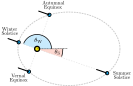
\includegraphics[width=0.6\linewidth]{solstice_angles.pdf}
  \caption{Orbital path with exaggerated eccentricity of Earth (blue) around
  the sun (yellow) with $\psi$ indicating an angular range either side of the
solstices in the sun centred ecliptic frame. The arrow extending from Earth
points in the direction of the north pole.}
  \label{fig:orbital_angles}
\end{figure}
However, it can be shown that the insolation experienced at latitude $\varphi$ over the orbital
range $\psi$ is the same as the insolation experienced on the opposite side of
the orbit, at latitude $-\varphi$ over the same range. This results in the annual average
insolation being symmetric about the equator.

To express insolation over the orbital range $\psi$, we integrate over
$\theta$, but also the longitude, $\gamma$. It is useful to separate our
expression for irradiance at a given point into two components, such that
\[
  I(r,\theta,\beta,\rho,\varphi,\gamma) =
  \frac{K}{4\pi r^2}S(\theta,\beta,\rho,\varphi,\gamma),
\]
where 
\[
  S(\theta,\beta,\rho,\varphi,\gamma) = (\sin{\gamma}\sin{(\rho -
  \theta)}-\cos{\beta} \cos{\gamma} \cos{(\rho-\theta)})\cos{\varphi}
  -\sin{\beta}\sin{\varphi} \cos{(\rho -\theta)}.
\]
The insolation over the range $\psi$, centred on the northern summer soltice is
therefore
\[
  Q_{\mathrm{N}} = \int_{t(\theta_{\mathrm{N}}-\frac{\psi}{2})}^{t(\theta_{\mathrm{N}}+\frac{\psi}{2})}
  \int_{\gamma_1}^{\gamma_2}
  \frac{K}{4\pi r^2} S(\theta,\beta,\rho,\varphi,\gamma)\, \mathrm{d}\gamma\,\mathrm{d}t,
\]
where $t(\theta)$ is the time that corresponds to orbital angle $\theta$. Note
that the longitudinal limits also depend on $\theta, \beta, \rho$, and
$\varphi$, which vary so as to only span the positive range of $S$. This is shown by the red
regions in Figure \ref{fig:gamma_limits}.

Changing the variable of integration to $\theta$, we obtain
\begin{align*}
    Q_{\mathrm{N}} &= \int_{\theta_{\mathrm{N}}-\frac{\psi}{2}}^{\theta_{\mathrm{N}}+\frac{\psi}{2}}
  \int_{\gamma_1}^{\gamma_2}
  \frac{K}{4\pi r^2}S(\theta,\beta,\rho,\varphi,\gamma)\,\mathrm{d}\gamma\,\frac{\mathrm{d}t}{\mathrm{d}\theta}\,\mathrm{d}\theta\\
  &=\int_{\theta_{\mathrm{N}}-\frac{\psi}{2}}^{\theta_{\mathrm{N}}+\frac{\psi}{2}}\int_{\gamma_1}^{\gamma_2}
  \frac{K}{4\pi r^2}\frac{Pr^2}{2\pi a b}S(\theta,\beta,\rho,\varphi,\gamma)\, \mathrm{d}\gamma\,\mathrm{d}\theta\\
  &=\frac{KP}{8\pi^2 a b}\int_{\theta_{\mathrm{N}}-\frac{\psi}{2}}^{\theta_{\mathrm{N}}+\frac{\psi}{2}} \int_{\gamma_1}^{\gamma_2}
  S(\theta,\beta,\rho,\varphi,\gamma)\, \mathrm{d}\gamma \,\mathrm{d}\theta\\
  &=\frac{KP}{8\pi^2 a b}\biggl[\Bigl[\gamma \sin{\beta} \sin{\varphi}
  \sin(\rho - \theta) \\
 &\quad\quad\quad\quad + (\sin{\gamma} \sin{(\rho - \theta)} \cos{\beta}
-\cos{\gamma}\cos(\rho - \theta))\cos{\varphi}\Bigr]_{\gamma_1}^{\gamma_2}
\biggr]_{\theta_{\mathrm{N}}-\frac{\psi}{2}}^{\theta_{\mathrm{N}}+\frac{\psi}{2}}\numberthis\label{eq:north_summer_solstice}
\end{align*}

\begin{figure}
  \centering
  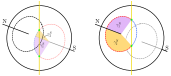
\includegraphics[width=0.9\linewidth]{gamma_limits.pdf}
  \caption{Two points during Earth's orbit from a top-down perspective in the
    ecliptic frame based on current orbital parameters. The two dashed
    circles in each plot lie at latitude $\varphi$ in the northern
    hemisphere and $-\varphi$ in the southern hemisphere. The case on the right 
    occurs when Earth is at its aphelion and the sun is to the left of the
    black dotted line. The longitudinal range of where the sun reaches the
    northern circle (red) spans from $\gamma_1$ to $\gamma_2$. The diagram on
    the left occurs when Earth is at its perihelion and the sun is to the
    right of the dotted line. Here the longitudinal limits are
  $\pi-\gamma_1$ and $\pi-\gamma_2$.}
  \label{fig:gamma_limits}
\end{figure}

If we now compare this to the same angle range of the orbit centred around the southern
hemisphere's summer solstice, at latitude $-\varphi$, we will see they are equivalent. 

The southern summer solstice occurs at an angle of $\theta_{\mathrm{N}}+\pi$.
This causes the range over which $S$ is positive to change, as shown in the left
diagram of Figure \ref{fig:gamma_limits}. Due to symmetry, the circles of
constant latitude in each hemisphere will experience an equal amount of
sunlight at opposite sides of the orbit. However, longitude is measured from
the same point throughout the orbit, where the north pole points in the
ecliptic $x$-$y$ plane. This means the longitudinal limits in the southern
hemisphere are offset to the northern hemisphere's limits by $\pi$.

Following the same steps as before, we find the insolation for the
southern hemisphere to be
\[
\begin{split}
  Q_{\mathrm{S}} &=\frac{KP}{8\pi^2 a b}\int_{\theta_{\mathrm{N}}+\pi-\frac{\psi}{2}}^{
  \theta_{\mathrm{N}}+\pi+\frac{\psi}{2}}\int_{\pi-\gamma_1}^{\pi-\gamma_2}S(\theta,
  \beta,\rho,-\varphi,\gamma)\,\mathrm{d}\gamma \,\mathrm{d}\theta\\
  &= \frac{KP}{8\pi^2 a b}\int_{\theta_{\mathrm{N}}-\frac{\psi}{2}}^{\theta_{\mathrm{N}}+\frac{\psi}{2}}
  \int_{\gamma_1}^{\gamma_2} S((\theta+\pi),\beta,\rho,-\varphi,(\pi-\gamma))\,
  \mathrm{d}\gamma \,\mathrm{d}\theta\\
  &= \frac{KP}{8\pi^2 a b}\biggl[\Bigl[(\gamma-\pi) \sin{\beta} \sin{\varphi}
  \sin(\rho - \theta) \\
  &\quad\quad\quad\quad+ (\sin{\gamma} \sin{(\rho - \theta)} \cos{\beta} -
\cos{\gamma} \cos(\rho - \theta))\cos{\varphi}\Bigr]_{\gamma_1}^{\gamma_2}
\biggr]_{\theta_{\mathrm{N}}-\frac{\psi}{2}}^{\theta_{\mathrm{N}}+\frac{\psi}{2}},
\end{split}
\]
where the only difference from (\ref{eq:north_summer_solstice}) is the
subtracted $\pi$ multiplying the first term, which disappears once the limits
for $\gamma$ are substituted in. 


\begin{figure}
  \centering
  \includegraphics[width=0.6\linewidth]{yearly_average_insol_150kN.pdf}
  \caption{Contour showing the difference in yearly average insolation from the
  average insolation over the 150k year period at each latitude. The lower
  plot shows how these fluctuations in yearly insolation correlate with Earth's
  obliquity.}
  \label{fig:yearly_ave_insol_all_lats}
\end{figure}

\bibliographystyle{ieeetr}
\bibliography{refs}
\end{document}
